\documentclass[10pt]{article}
\usepackage{amsmath,amsfonts,times}
\usepackage{graphicx,color,tikz,pgfplots}
\usepackage[paperwidth=16.5cm,paperheight=5.5cm,lmargin=0in,rmargin=0in,tmargin=0.in,bmargin=0.in]{geometry}
\usepackage{bm}
\usetikzlibrary{arrows,shadings,shapes.arrows,decorations.pathreplacing,calc, positioning}
\usepgfplotslibrary{fillbetween}

\pgfplotsset{
  compat=newest
}

\newlength{\dx}
\setlength{\dx}{0.8cm}

\newlength{\circleRadius}
\setlength{\circleRadius}{0.95\dx}

\definecolor{outside}{rgb}{0, 1, 0}
\definecolor{cutcell}{rgb}{0, 0.5, 1}
\definecolor{inside}{rgb}{1, 0, 0}

\tikzset{
  circ/.style={very thick, draw=black},
  outline/.style={thick, draw=black, densely dashed, fill=gray!25!white}
}

\begin{document}
\centering
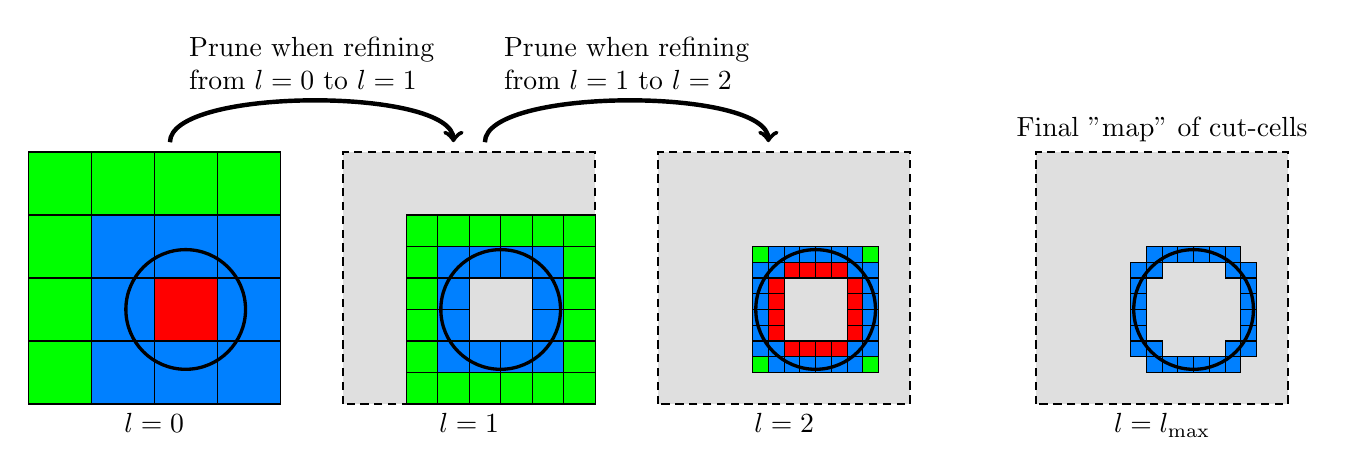
\begin{tikzpicture}
%  \draw[step=\dx] (0,0) grid (4\dx, 4\dx);
  \draw[draw=black, fill=outside] (0,0) rectangle ++(\dx, \dx);
  \draw[draw=black, fill=outside] (0,\dx) rectangle ++(\dx, \dx);
  \draw[draw=black, fill=outside] (0,2\dx) rectangle ++(\dx, \dx);
  \draw[draw=black, fill=outside] (0,3\dx) rectangle ++(\dx, \dx);

  \draw[draw=black, fill=cutcell] (\dx,0) rectangle ++(\dx, \dx);
  \draw[draw=black, fill=cutcell] (\dx,\dx) rectangle ++(\dx, \dx);
  \draw[draw=black, fill=cutcell] (\dx,2\dx) rectangle ++(\dx, \dx);
  \draw[draw=black, fill=outside] (\dx,3\dx) rectangle ++(\dx, \dx);

  \draw[draw=black, fill=cutcell] (2\dx,0) rectangle ++(\dx, \dx);
  \draw[draw=black, fill=inside] (2\dx,\dx) rectangle ++(\dx, \dx);
  \draw[draw=black, fill=cutcell] (2\dx,2\dx) rectangle ++(\dx, \dx);
  \draw[draw=black, fill=outside] (2\dx,3\dx) rectangle ++(\dx, \dx);

  \draw[draw=black, fill=cutcell] (3\dx,0) rectangle ++(\dx, \dx);
  \draw[draw=black, fill=cutcell] (3\dx,\dx) rectangle ++(\dx, \dx);
  \draw[draw=black, fill=cutcell] (3\dx,2\dx) rectangle ++(\dx, \dx);
  \draw[draw=black, fill=outside] (3\dx,3\dx) rectangle ++(\dx, \dx);

  \draw[circ] (2.5\dx,1.5\dx) circle (\circleRadius);

  \begin{scope}[xshift=5\dx]
    \draw[outline] (0,0) rectangle (4\dx, 4\dx);
%    \draw[step=0.5\dx] (0,0) grid (4\dx, 4\dx);
    \draw[draw=black, fill=outside] (\dx,0) rectangle ++(0.5\dx, 0.5\dx);
    \draw[draw=black, fill=outside] (1.5\dx,0) rectangle ++(0.5\dx, 0.5\dx);
    \draw[draw=black, fill=outside] (\dx,0.5\dx) rectangle ++(0.5\dx, 0.5\dx);
    \draw[draw=black, fill=cutcell] (1.5\dx,0.5\dx) rectangle ++(0.5\dx, 0.5\dx);
    
    \draw[draw=black, fill=outside] (\dx,\dx) rectangle ++(0.5\dx, 0.5\dx);
    \draw[draw=black, fill=cutcell] (1.5\dx,\dx) rectangle ++(0.5\dx, 0.5\dx);
    \draw[draw=black, fill=outside] (\dx,1.5\dx) rectangle ++(0.5\dx, 0.5\dx);
    \draw[draw=black, fill=cutcell] (1.5\dx,1.5\dx) rectangle ++(0.5\dx, 0.5\dx);
    
    \draw[draw=black, fill=outside] (\dx,2\dx) rectangle ++(0.5\dx, 0.5\dx);
    \draw[draw=black, fill=cutcell] (1.5\dx,2\dx) rectangle ++(0.5\dx, 0.5\dx);
    \draw[draw=black, fill=outside] (\dx,2.5\dx) rectangle ++(0.5\dx, 0.5\dx);
    \draw[draw=black, fill=outside] (1.5\dx,2.5\dx) rectangle ++(0.5\dx, 0.5\dx);

    \draw[draw=black, fill=outside] (2\dx,0) rectangle ++(0.5\dx, 0.5\dx);
    \draw[draw=black, fill=outside] (2.5\dx,0) rectangle ++(0.5\dx, 0.5\dx);
    \draw[draw=black, fill=cutcell] (2\dx,0.5\dx) rectangle ++(0.5\dx, 0.5\dx);
    \draw[draw=black, fill=cutcell] (2.5\dx,0.5\dx) rectangle ++(0.5\dx, 0.5\dx);

    \draw[draw=black, fill=cutcell] (2\dx,2\dx) rectangle ++(0.5\dx, 0.5\dx);
    \draw[draw=black, fill=cutcell] (2.5\dx,2\dx) rectangle ++(0.5\dx, 0.5\dx);
    \draw[draw=black, fill=outside] (2\dx,2.5\dx) rectangle ++(0.5\dx, 0.5\dx);
    \draw[draw=black, fill=outside] (2.5\dx,2.5\dx) rectangle ++(0.5\dx, 0.5\dx);

    \draw[draw=black, fill=outside] (3\dx,0) rectangle ++(0.5\dx, 0.5\dx);
    \draw[draw=black, fill=outside] (3.5\dx,0) rectangle ++(0.5\dx, 0.5\dx);
    \draw[draw=black, fill=cutcell] (3\dx,0.5\dx) rectangle ++(0.5\dx, 0.5\dx);
    \draw[draw=black, fill=outside] (3.5\dx,0.5\dx) rectangle ++(0.5\dx, 0.5\dx);
    
    \draw[draw=black, fill=cutcell] (3\dx,\dx) rectangle ++(0.5\dx, 0.5\dx);
    \draw[draw=black, fill=outside] (3.5\dx,\dx) rectangle ++(0.5\dx, 0.5\dx);
    \draw[draw=black, fill=cutcell] (3\dx,1.5\dx) rectangle ++(0.5\dx, 0.5\dx);
    \draw[draw=black, fill=outside] (3.5\dx,1.5\dx) rectangle ++(0.5\dx, 0.5\dx);
    
    \draw[draw=black, fill=cutcell] (3\dx,2\dx) rectangle ++(0.5\dx, 0.5\dx);
    \draw[draw=black, fill=outside] (3.5\dx,2\dx) rectangle ++(0.5\dx, 0.5\dx);
    \draw[draw=black, fill=outside] (3\dx,2.5\dx) rectangle ++(0.5\dx, 0.5\dx);
    \draw[draw=black, fill=outside] (3.5\dx,2.5\dx) rectangle ++(0.5\dx, 0.5\dx);

    % Stuff from elsewhere
    %% \draw[draw=black, fill=outside] (0,0) rectangle ++(\dx, \dx);
    %% \draw[draw=black, fill=outside] (0,\dx) rectangle ++(\dx, \dx);
    %% \draw[draw=black, fill=outside] (0,2\dx) rectangle ++(\dx, \dx);
    %% \draw[draw=black, fill=outside] (0,3\dx) rectangle ++(\dx, \dx);
    %% \draw[draw=black, fill=inside] (2\dx,\dx) rectangle ++(\dx, \dx);
    %% \draw[draw=black, fill=outside] (\dx,3\dx) rectangle ++(\dx, \dx);
    %% \draw[draw=black, fill=outside] (2\dx,3\dx) rectangle ++(\dx, \dx);
    %% \draw[draw=black, fill=outside] (3\dx,3\dx) rectangle ++(\dx, \dx);

    % Circle
    \draw[circ] (2.5\dx,1.5\dx) circle (\circleRadius);
  \end{scope}

  \begin{scope}[xshift=10\dx]
    \draw[outline] (0,0) rectangle (4\dx, 4\dx);
%    \draw[step=0.25\dx] (0,0) grid (4\dx, 4\dx);
    \draw[draw=black, fill=outside] (1.5\dx,0.5\dx) rectangle ++(0.25\dx, 0.25\dx);
    \draw[draw=black, fill=cutcell] (1.75\dx,0.5\dx) rectangle ++(0.25\dx, 0.25\dx);
    \draw[draw=black, fill=cutcell] (1.5\dx,0.75\dx) rectangle ++(0.25\dx, 0.25\dx);
    \draw[draw=black, fill=cutcell] (1.75\dx,0.75\dx) rectangle ++(0.25\dx, 0.25\dx);
    
    \draw[draw=black, fill=cutcell] (1.5\dx,\dx) rectangle ++(0.25\dx, 0.25\dx);
    \draw[draw=black, fill=inside] (1.75\dx,\dx) rectangle ++(0.25\dx, 0.25\dx);
    \draw[draw=black, fill=cutcell] (1.5\dx,1.25\dx) rectangle ++(0.25\dx, 0.25\dx);
    \draw[draw=black, fill=inside] (1.75\dx,1.25\dx) rectangle ++(0.25\dx, 0.25\dx);
    
    \draw[draw=black, fill=cutcell] (1.5\dx,1.5\dx) rectangle ++(0.25\dx, 0.25\dx);
    \draw[draw=black, fill=inside] (1.75\dx,1.5\dx) rectangle ++(0.25\dx, 0.25\dx);
    \draw[draw=black, fill=cutcell] (1.5\dx,1.75\dx) rectangle ++(0.25\dx, 0.25\dx);
    \draw[draw=black, fill=inside] (1.75\dx,1.75\dx) rectangle ++(0.25\dx, 0.25\dx);
    
    \draw[draw=black, fill=cutcell] (1.5\dx,2\dx) rectangle ++(0.25\dx, 0.25\dx);
    \draw[draw=black, fill=cutcell] (1.75\dx,2\dx) rectangle ++(0.25\dx, 0.25\dx);
    \draw[draw=black, fill=outside] (1.5\dx,2.25\dx) rectangle ++(0.25\dx, 0.25\dx);
    \draw[draw=black, fill=cutcell] (1.75\dx,2.25\dx) rectangle ++(0.25\dx, 0.25\dx);

    \draw[draw=black, fill=cutcell] (2\dx,0.5\dx) rectangle ++(0.25\dx, 0.25\dx);
    \draw[draw=black, fill=cutcell] (2.25\dx,0.5\dx) rectangle ++(0.25\dx, 0.25\dx);
    \draw[draw=black, fill=inside] (2\dx,0.75\dx) rectangle ++(0.25\dx, 0.25\dx);
    \draw[draw=black, fill=inside] (2.25\dx,0.75\dx) rectangle ++(0.25\dx, 0.25\dx);
    
    \draw[draw=black, fill=cutcell] (2.5\dx,0.5\dx) rectangle ++(0.25\dx, 0.25\dx);
    \draw[draw=black, fill=cutcell] (2.75\dx,0.5\dx) rectangle ++(0.25\dx, 0.25\dx);
    \draw[draw=black, fill=inside] (2.5\dx,0.75\dx) rectangle ++(0.25\dx, 0.25\dx);
    \draw[draw=black, fill=inside] (2.75\dx,0.75\dx) rectangle ++(0.25\dx, 0.25\dx);

    \draw[draw=black, fill=inside] (2\dx,2\dx) rectangle ++(0.25\dx, 0.25\dx);
    \draw[draw=black, fill=inside] (2.25\dx,2\dx) rectangle ++(0.25\dx, 0.25\dx);
    \draw[draw=black, fill=cutcell] (2\dx,2.25\dx) rectangle ++(0.25\dx, 0.25\dx);
    \draw[draw=black, fill=cutcell] (2.25\dx,2.25\dx) rectangle ++(0.25\dx, 0.25\dx);
    
    \draw[draw=black, fill=inside] (2.5\dx,2\dx) rectangle ++(0.25\dx, 0.25\dx);
    \draw[draw=black, fill=inside] (2.75\dx,2\dx) rectangle ++(0.25\dx, 0.25\dx);
    \draw[draw=black, fill=cutcell] (2.5\dx,2.25\dx) rectangle ++(0.25\dx, 0.25\dx);
    \draw[draw=black, fill=cutcell] (2.75\dx,2.25\dx) rectangle ++(0.25\dx, 0.25\dx);

    \draw[draw=black, fill=cutcell] (3\dx,0.5\dx) rectangle ++(0.25\dx, 0.25\dx);
    \draw[draw=black, fill=outside] (3.25\dx,0.5\dx) rectangle ++(0.25\dx, 0.25\dx);
    \draw[draw=black, fill=cutcell] (3\dx,0.75\dx) rectangle ++(0.25\dx, 0.25\dx);
    \draw[draw=black, fill=cutcell] (3.25\dx,0.75\dx) rectangle ++(0.25\dx, 0.25\dx);
    
    \draw[draw=black, fill=inside] (3\dx,\dx) rectangle ++(0.25\dx, 0.25\dx);
    \draw[draw=black, fill=cutcell] (3.25\dx,\dx) rectangle ++(0.25\dx, 0.25\dx);
    \draw[draw=black, fill=inside] (3\dx,1.25\dx) rectangle ++(0.25\dx, 0.25\dx);
    \draw[draw=black, fill=cutcell] (3.25\dx,1.25\dx) rectangle ++(0.25\dx, 0.25\dx);
    
    \draw[draw=black, fill=inside] (3\dx,1.5\dx) rectangle ++(0.25\dx, 0.25\dx);
    \draw[draw=black, fill=cutcell] (3.25\dx,1.5\dx) rectangle ++(0.25\dx, 0.25\dx);
    \draw[draw=black, fill=inside] (3\dx,1.75\dx) rectangle ++(0.25\dx, 0.25\dx);
    \draw[draw=black, fill=cutcell] (3.25\dx,1.75\dx) rectangle ++(0.25\dx, 0.25\dx);
    
    \draw[draw=black, fill=cutcell] (3\dx,2\dx) rectangle ++(0.25\dx, 0.25\dx);
    \draw[draw=black, fill=cutcell] (3.25\dx,2\dx) rectangle ++(0.25\dx, 0.25\dx);
    \draw[draw=black, fill=cutcell] (3\dx,2.25\dx) rectangle ++(0.25\dx, 0.25\dx);
    \draw[draw=black, fill=outside] (3.25\dx,2.25\dx) rectangle ++(0.25\dx, 0.25\dx);
    
    \draw[circ] (2.5\dx,1.5\dx) circle (\circleRadius);
  \end{scope}

  \begin{scope}[xshift=16\dx]
    \draw[outline] (0,0) rectangle (4\dx, 4\dx);
%    \draw[step=0.25\dx] (0,0) grid (4\dx, 4\dx);
    \draw[draw=black, fill=cutcell] (1.75\dx,0.5\dx) rectangle ++(0.25\dx, 0.25\dx);
    \draw[draw=black, fill=cutcell] (1.5\dx,0.75\dx) rectangle ++(0.25\dx, 0.25\dx);
    \draw[draw=black, fill=cutcell] (1.75\dx,0.75\dx) rectangle ++(0.25\dx, 0.25\dx);
    
    \draw[draw=black, fill=cutcell] (1.5\dx,\dx) rectangle ++(0.25\dx, 0.25\dx);
    \draw[draw=black, fill=cutcell] (1.5\dx,1.25\dx) rectangle ++(0.25\dx, 0.25\dx);
    
    \draw[draw=black, fill=cutcell] (1.5\dx,1.5\dx) rectangle ++(0.25\dx, 0.25\dx);
    \draw[draw=black, fill=cutcell] (1.5\dx,1.75\dx) rectangle ++(0.25\dx, 0.25\dx);
    
    \draw[draw=black, fill=cutcell] (1.5\dx,2\dx) rectangle ++(0.25\dx, 0.25\dx);
    \draw[draw=black, fill=cutcell] (1.75\dx,2\dx) rectangle ++(0.25\dx, 0.25\dx);
    \draw[draw=black, fill=cutcell] (1.75\dx,2.25\dx) rectangle ++(0.25\dx, 0.25\dx);

    \draw[draw=black, fill=cutcell] (2\dx,0.5\dx) rectangle ++(0.25\dx, 0.25\dx);
    \draw[draw=black, fill=cutcell] (2.25\dx,0.5\dx) rectangle ++(0.25\dx, 0.25\dx);
    
    \draw[draw=black, fill=cutcell] (2.5\dx,0.5\dx) rectangle ++(0.25\dx, 0.25\dx);
    \draw[draw=black, fill=cutcell] (2.75\dx,0.5\dx) rectangle ++(0.25\dx, 0.25\dx);

    \draw[draw=black, fill=cutcell] (2\dx,2.25\dx) rectangle ++(0.25\dx, 0.25\dx);
    \draw[draw=black, fill=cutcell] (2.25\dx,2.25\dx) rectangle ++(0.25\dx, 0.25\dx);
    
    \draw[draw=black, fill=cutcell] (2.5\dx,2.25\dx) rectangle ++(0.25\dx, 0.25\dx);
    \draw[draw=black, fill=cutcell] (2.75\dx,2.25\dx) rectangle ++(0.25\dx, 0.25\dx);

    \draw[draw=black, fill=cutcell] (3\dx,0.5\dx) rectangle ++(0.25\dx, 0.25\dx);
    \draw[draw=black, fill=cutcell] (3\dx,0.75\dx) rectangle ++(0.25\dx, 0.25\dx);
    \draw[draw=black, fill=cutcell] (3.25\dx,0.75\dx) rectangle ++(0.25\dx, 0.25\dx);
    
    \draw[draw=black, fill=cutcell] (3.25\dx,\dx) rectangle ++(0.25\dx, 0.25\dx);
    \draw[draw=black, fill=cutcell] (3.25\dx,1.25\dx) rectangle ++(0.25\dx, 0.25\dx);
    
    \draw[draw=black, fill=cutcell] (3.25\dx,1.5\dx) rectangle ++(0.25\dx, 0.25\dx);
    \draw[draw=black, fill=cutcell] (3.25\dx,1.75\dx) rectangle ++(0.25\dx, 0.25\dx);
    
    \draw[draw=black, fill=cutcell] (3\dx,2\dx) rectangle ++(0.25\dx, 0.25\dx);
    \draw[draw=black, fill=cutcell] (3.25\dx,2\dx) rectangle ++(0.25\dx, 0.25\dx);
    \draw[draw=black, fill=cutcell] (3\dx,2.25\dx) rectangle ++(0.25\dx, 0.25\dx);
    
    \draw[circ] (2.5\dx,1.5\dx) circle (\circleRadius);
  \end{scope}

  \node[alias=a] at (2.25\dx,4\dx) {};
  \node[alias=b] at (6.75\dx,4\dx) {};
  \node[alias=c] at (7.25\dx,4\dx) {};
  \node[alias=d] at (11.75\dx,4\dx) {};

  \node[anchor=north] at (2\dx,0\dx) {$l=0$};
  \node[anchor=north] at (7\dx,0\dx) {$l=1$};
  \node[anchor=north] at (12\dx,0\dx) {$l=2$};
  \node[anchor=north] at (18\dx,0\dx) {$l = l_{\textrm{max}}$};

  \node[anchor=south] at (18\dx,4\dx) {Final ''map'' of cut-cells};
  
  \draw[ultra thick, ->] (a) to[out=90, in=90, looseness=0.5] node[align=left, midway, above, minimum width=6\dx]{Prune when refining \\ from $l=0$ to $l=1$} (b);
  \draw[ultra thick, ->] (c) to[out=90, in=90, looseness=0.5] node[align=left, midway, above, minimum width=6\dx]{Prune when refining \\ from $l=1$ to $l=2$} (d);
  
\end{tikzpicture}

\end{document} 
